\documentclass[tikz,border=8pt]{standalone}
% Shared look for every TikZ diagram. Load with % Shared look for every TikZ diagram. Load with % Shared look for every TikZ diagram. Load with \input{../../tools/tikz-style.tex}
\usepackage[T1]{fontenc}
\usepackage{lmodern}
\renewcommand{\sfdefault}{lmr}  % diagrams use the same serif as the text
\usetikzlibrary{arrows.meta, positioning, shapes.geometric, calc, fit, backgrounds}
\definecolor{cblue}{HTML}{4C78A8}
\definecolor{corange}{HTML}{F58518}
\definecolor{cgreen}{HTML}{54A24B}
\definecolor{cred}{HTML}{E45756}
\definecolor{cpurple}{HTML}{B279A2}
\definecolor{cgrey}{HTML}{6B6B6B}
\tikzset{
  every picture/.style={font=\sffamily, line width=1.2pt},
  box/.style={draw=#1, fill=#1!12, rounded corners=4pt, align=center, inner sep=7pt, minimum height=1.1cm},
  box/.default=cgrey,
  arrow/.style={-{Stealth[length=3mm]}, draw=cgrey, line width=1.4pt},
  title/.style={font=\sffamily\bfseries\Large},
  note/.style={font=\sffamily\small, text=cgrey, align=center},
}
\AtBeginDocument{\hyphenpenalty=10000 \exhyphenpenalty=10000}

\usepackage[T1]{fontenc}
\usepackage{lmodern}
\renewcommand{\sfdefault}{lmr}  % diagrams use the same serif as the text
\usetikzlibrary{arrows.meta, positioning, shapes.geometric, calc, fit, backgrounds}
\definecolor{cblue}{HTML}{4C78A8}
\definecolor{corange}{HTML}{F58518}
\definecolor{cgreen}{HTML}{54A24B}
\definecolor{cred}{HTML}{E45756}
\definecolor{cpurple}{HTML}{B279A2}
\definecolor{cgrey}{HTML}{6B6B6B}
\tikzset{
  every picture/.style={font=\sffamily, line width=1.2pt},
  box/.style={draw=#1, fill=#1!12, rounded corners=4pt, align=center, inner sep=7pt, minimum height=1.1cm},
  box/.default=cgrey,
  arrow/.style={-{Stealth[length=3mm]}, draw=cgrey, line width=1.4pt},
  title/.style={font=\sffamily\bfseries\Large},
  note/.style={font=\sffamily\small, text=cgrey, align=center},
}
\AtBeginDocument{\hyphenpenalty=10000 \exhyphenpenalty=10000}

\usepackage[T1]{fontenc}
\usepackage{lmodern}
\renewcommand{\sfdefault}{lmr}  % diagrams use the same serif as the text
\usetikzlibrary{arrows.meta, positioning, shapes.geometric, calc, fit, backgrounds}
\definecolor{cblue}{HTML}{4C78A8}
\definecolor{corange}{HTML}{F58518}
\definecolor{cgreen}{HTML}{54A24B}
\definecolor{cred}{HTML}{E45756}
\definecolor{cpurple}{HTML}{B279A2}
\definecolor{cgrey}{HTML}{6B6B6B}
\tikzset{
  every picture/.style={font=\sffamily, line width=1.2pt},
  box/.style={draw=#1, fill=#1!12, rounded corners=4pt, align=center, inner sep=7pt, minimum height=1.1cm},
  box/.default=cgrey,
  arrow/.style={-{Stealth[length=3mm]}, draw=cgrey, line width=1.4pt},
  title/.style={font=\sffamily\bfseries\Large},
  note/.style={font=\sffamily\small, text=cgrey, align=center},
}
\AtBeginDocument{\hyphenpenalty=10000 \exhyphenpenalty=10000}

\begin{document}
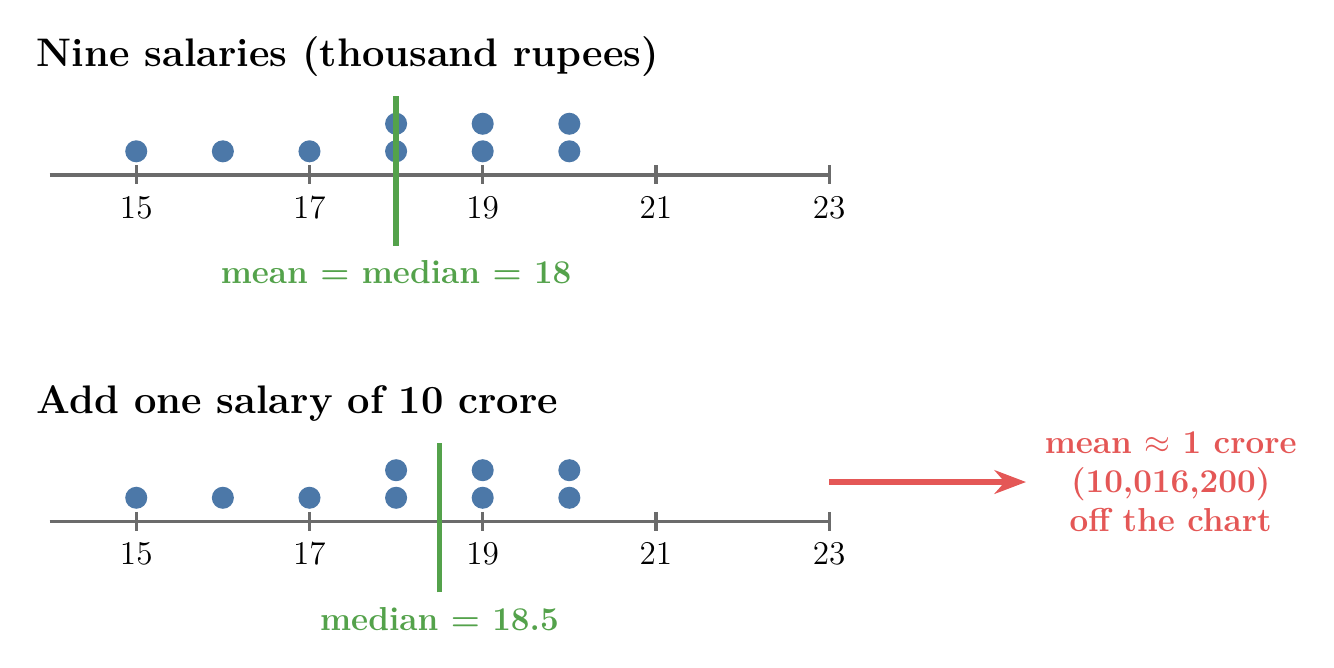
\begin{tikzpicture}[every node/.append style={font=\sffamily\large}]
\tikzset{note/.style={font=\sffamily\large, text=cgrey, align=center}}
  % scale: x = (salary - 14000)/1000 * 1.1
  \def\sx#1{(#1-14)*1.1}
  \node[title, anchor=west] at (-0.3,1.5) {Nine salaries (thousand rupees)};
  \draw[cgrey] (0,0) -- (9.9,0);
  \foreach \t in {15,17,...,23} { \draw[cgrey] ({\sx{\t}},0.12) -- ({\sx{\t}},-0.12); \node[below, font=\sffamily\large] at ({\sx{\t}},-0.15) {\t}; }
  \foreach \v/\k in {15/0,16/0,17/0,18/0,18/1,19/0,19/1,20/0,20/1} \fill[cblue] ({\sx{\v}},0.3+0.35*\k) circle (0.14);
  \draw[cgreen, line width=2pt] ({\sx{18}},-0.9) -- ({\sx{18}},1.0);
  \node[text=cgreen, font=\sffamily\bfseries\large, anchor=north] at ({\sx{18}},-0.95) {mean = median = 18};
  \begin{scope}[yshift=-4.4cm]
  \node[title, anchor=west] at (-0.3,1.5) {Add one salary of 10 crore};
  \draw[cgrey] (0,0) -- (9.9,0);
  \foreach \t in {15,17,...,23} { \draw[cgrey] ({\sx{\t}},0.12) -- ({\sx{\t}},-0.12); \node[below, font=\sffamily\large] at ({\sx{\t}},-0.15) {\t}; }
  \foreach \v/\k in {15/0,16/0,17/0,18/0,18/1,19/0,19/1,20/0,20/1} \fill[cblue] ({\sx{\v}},0.3+0.35*\k) circle (0.14);
  \draw[cgreen, line width=2pt] ({\sx{18.5}},-0.9) -- ({\sx{18.5}},1.0);
  \node[text=cgreen, font=\sffamily\bfseries\large, anchor=north] at ({\sx{18.5}},-0.95) {median = 18.5};
  \draw[cred, line width=2pt, -{Stealth[length=4mm]}] (9.9,0.5) -- (12.4,0.5);
  \node[text=cred, font=\sffamily\bfseries\large, align=center, anchor=west] at (12.5,0.5) {mean $\approx$ 1 crore\\(10,016,200)\\off the chart};
  \end{scope}
\end{tikzpicture}
\end{document}
